% AAAI'27-style course report for BGU course 237-2-5513.
% Official, unmodified style assets are documented in
% AAAI27_AUTHOR_KIT_PROVENANCE.md.  The course instructions recommend
% camera-ready formatting and \nocopyright for this submission.
\documentclass[letterpaper]{article}
\usepackage{aaai2027}
\usepackage[hyphens]{url}
\usepackage{graphicx}
\usepackage{natbib}
\usepackage{amsmath,amssymb}
\usepackage{booktabs}
\urlstyle{rm}
\def\UrlFont{\rm}
\frenchspacing

\pdfinfo{
/TemplateVersion (2027.1)
}
\nocopyright
\setcounter{secnumdepth}{0}
\graphicspath{{generated/}}

\newcommand{\Astar}{A$^\ast$}
\newcommand{\HMan}{\ensuremath{H_0}}
\newcommand{\HPrefix}{\ensuremath{H_4}}
\newcommand{\HFull}{\ensuremath{H_{32}}}
\newcommand{\Staged}{\textsc{Staged}}
\newcommand{\LazyFull}{\textsc{Lazy-Full}}
\newcommand{\EagerFull}{\textsc{Eager-Full}}
\newcommand{\Manhattan}{\textsc{Manhattan}}

\title{Progressive Landmark Evaluation in \Astar{}:\\
An Empirical Study of Nested Differential Heuristics}
\author{\textbf{Nevo Levi (ID: 207350646)} \qquad
        \textbf{Dvir Chitrit (ID: 206766818)}}
\affiliations{\small
  Ben-Gurion University of the Negev --- Course 237-2-5513:
  Search Methods in Artificial Intelligence
}

\begin{document}
\maketitle

\begin{abstract}
Differential landmarks give strong admissible estimates but require many
table reads.  Lazy \Astar{} avoids some of this work by evaluating the full
heuristic only when a state becomes competitive in OPEN.  We ask whether a
fixed intermediate prefix can avoid still more landmark work: states first
receive Manhattan distance, then four landmark terms, and only then the
remaining terms of a 32-landmark heuristic.  We compare Manhattan, eager
full-landmark, ordinary lazy full-landmark, and staged evaluation in a shared
optimal graph-search implementation.  The map-disjoint evaluation contains
800 queries over eight Moving AI maps from four topology families, with one
warm-up and eight position-balanced timed repetitions per method and query.
All returned costs matched independent BFS, and eager, lazy, and staged full
landmark search had identical expansion traces on all 800 queries.  Staging
saved a median 3.10\% of pivot evaluations and 3.02\% of distance-table reads
relative to ordinary lazy evaluation, but its primary median paired time ratio
was 1.0543 (staged/lazy; hierarchical 95\% bootstrap interval
$[0.9890,1.1016]$).  Its descriptive bootstrap probability of a ratio below
one was 0.053.  The crossover was strongly regime-dependent: both maze maps
favored staging, whereas both warehouse maps had zero median read saving and
favored ordinary lazy evaluation.  Thus the extra OPEN cycle can erase a real
reduction in heuristic work; a fixed prefix is useful only when it filters
enough full evaluations.  The contribution is this controlled empirical
combination and mechanism decomposition, not a claim to invent landmarks,
subsets, or multi-stage Lazy \Astar{}.
\end{abstract}

\section{Introduction}
\label{sec:introduction}

Heuristics save search only after their own computational cost is paid.  This
tension is easy to hide when heuristic evaluation is treated as a constant:
a more informed admissible estimate generally expands no more states under a
fixed ordering, but it may still take longer to solve a problem.  Landmark
heuristics make the tradeoff concrete.  A preprocessing pass stores exact
distances from selected pivots; a query then obtains lower bounds from the
triangle inequality.  More pivots can strengthen the maximum, but each
evaluated state performs more table reads.

Lazy \Astar{} changes when this cost is paid.  A newly discovered state first
receives a cheap bound.  Only if it rises to the top of OPEN is an expensive
bound computed and the state reinserted; surplus states may never receive the
expensive heuristic \citep{tolpin2013towards,karpas2018rational}.  The saved
heuristic calls compete with extra priority-queue operations.  With a set of
32 differential landmarks, there is a natural intermediate design: compute a
fixed four-landmark prefix at the first competitive pop, and compute the other
28 terms only if the state remains competitive at a later pop.

This is a deliberately bounded course project.  It stays within optimal
single-agent \Astar{}, admissible and consistent heuristics, OPEN-list
behavior, and empirical comparison---the core material of a search-methods
course.  The extension adds no learned selector, calibration phase, rational
bypass, multi-agent solver, or new domain.  Its research question is narrow:
\emph{does an intermediate fixed landmark prefix save enough remaining
heuristic work to justify another OPEN cycle, and in which map regimes?}

We answer that question under a prospectively fixed protocol.  Four methods
share one deterministic graph-search engine: Manhattan distance,
eager evaluation of 32 landmarks, ordinary Lazy \Astar{} from Manhattan to all
32 landmarks, and progressive evaluation from Manhattan to four and then 32
landmarks.  The prefix and full counts are fixed at $K=4$ and $M=32$; no
development outcome selects them.  Twelve checksum-pinned Moving AI maps
define a map-disjoint split: four development maps authorize the unchanged
run, and eight sealed maps supply the reported 800-query evaluation.  Timing
uses rotated blocks in which every method occurs twice in every order
position.

The central result is a mechanism/performance split.  The staged method did
less deterministic landmark work: median pivot and read savings were 3.10\%
and 3.02\% relative to ordinary lazy evaluation.  Nevertheless, its median
paired time ratio was 1.0543, with a map-hierarchical 95\% bootstrap interval
from 0.9890 to 1.1016.  Savings and timing varied by topology.  Both maze maps
had substantial landmark savings and staged/lazy ratios below one; both
warehouse maps had zero median savings and ratios above one.  Across queries,
read saving and log time ratio had descriptive Spearman correlation
$\rho=-0.6406$, consistent with a crossover but not identifying a causal
effect.

The paper contributes (i) a fully specified three-level evaluation schedule
for a nested differential heuristic; (ii) a correctness argument and a
trace-invariance gate that separates scheduling from search order; and (iii)
a reproducible, map-disjoint decomposition of saved pivot work, extra OPEN
work, runtime, and preprocessing amortization.  The novelty boundary is
intentionally modest.  Landmark lower bounds, differential heuristics,
heuristic subsets, Lazy \Astar{}, and extension to more than two stages are
prior ideas.  A targeted literature search did not locate this exact fixed-
prefix, node-level staging experiment; that is not an exhaustive priority
claim.

\section{Background and Related Work}
\label{sec:related}

\paragraph{Optimal heuristic search.}
\Astar{} orders search states by $f(n)=g(n)+h(n)$, where $g$ is path cost and
$h$ estimates remaining cost \citep{hart1968formal}.  An admissible heuristic
never exceeds the true remaining cost; consistency additionally requires
$h(n)\leq c(n,n')+h(n')$ for every edge.  These properties and the details of
graph search, reopening, and tie breaking matter to optimality and comparisons
of expansion behavior \citep{dechter1985generalized}.  Our implementation
uses only lower-bound keys, supports reopening, and makes all final-stage
ordering deterministic.

\paragraph{Landmarks and differential heuristics.}
ALT uses exact distances to selected landmarks with triangle inequalities to
accelerate shortest-path search \citep{goldberg2005computing}.  For an
undirected graph, a differential heuristic takes
$|d(\ell,n)-d(\ell,t)|$ and maximizes over pivots
\citep{sturtevant2009memory}.  Landmark placement, count, memory, and
preprocessing are therefore established design dimensions, not contributions
of this project.  Likewise, selecting a fixed subset from many admissible
heuristics has been studied directly \citep{rayner2013subset}.  We lock a
deterministic farthest-first order and evaluate its first four members as an
intermediate stage; we do not optimize a subset on the reported maps.

\paragraph{Lazy and selective deployment.}
Lazy \Astar{} initially keys a generated state with a cheap heuristic and
computes an expensive heuristic only when that state becomes competitive in
OPEN.  The start is fully evaluated, and a valid popped goal is accepted
before unnecessary refinement \citep{tolpin2013towards}.  Rational Lazy
\Astar{} may bypass a costly evaluation using estimated usefulness and cost;
the archival treatment develops contextual rational deployment more broadly
\citep{karpas2018rational}.  Selective Max instead learns which heuristic to
evaluate \citep{domshlak2010max,domshlak2012online}.  Our schedule is neither
rational nor learned: every non-goal state must reach the complete 32-pivot
bound before expansion.  The Lazy \Astar{} literature describes extension to
multiple heuristic stages as straightforward.  Consequently, adding a third
stage alone is not an algorithmic novelty claim.

Dynamic-heuristic work gives a broader formal setting for refining estimates
during optimal search \citep{christen2025dynamic}.  We use the simpler nested,
consistent case.  Each promotion preserves or raises the key, and every
fully expanded state uses the same final heuristic.  This structure lets us
test a stronger invariant than cost equality: eager, ordinary lazy, and
staged full-landmark modes should enumerate successors in exactly the same
order.

\paragraph{Position of this study.}
Prior work establishes all ingredients separately: landmark preprocessing,
differential maxima, subset selection, lazy evaluation, and multi-stage
extension.  Our residual contribution is empirical.  We combine a fixed
four-pivot prefix with a fixed 32-pivot final bound, then measure whether
suffix calls avoided on surplus nodes outweigh the added requeues and pops.
This mechanism-first scope resembles the course's example projects, which
is useful pedagogically, but algorithmic facts and novelty boundaries here
are supported by the primary literature rather than by course examples.

\section{Questions and Hypotheses}
\label{sec:questions}

The study has four research questions.

\begin{description}
  \item[RQ1: Correctness and control.] Do all four modes return the independent
  BFS cost, and do the three modes that ultimately use \HFull{} have identical
  successor-expansion traces?

  \item[RQ2: Mechanism.] Relative to \LazyFull{}, how many pivot evaluations,
  distance-table reads, and suffix calls does \Staged{} avoid, and how many
  additional OPEN operations does it introduce?

  \item[RQ3: Search time.] What is the paired staged/lazy search-time ratio
  over map-disjoint evaluation queries, with maps rather than timing
  repetitions treated as the top-level independent units?

  \item[RQ4: Regimes and amortization.] How do the mechanism and timing ratio
  vary across maze, random, room, and warehouse maps, and how does one-time
  landmark construction affect total cost at different query volumes?
\end{description}

The prospectively encoded analysis maps these questions to three hypotheses.
H1 is a hard gate: all 800 sealed queries must pass BFS equality and
full-landmark trace invariance before timing is analyzed.  H2 expects staged
evaluation to save exact pivot evaluations and distance reads relative to
ordinary lazy evaluation.  H3 evaluates the paired time ratio and the
association between saved work and time; it is explicitly descriptive.  In
particular, the bootstrap fraction of replicates with a ratio below one is
not treated as a frequentist $p$-value, and the Spearman coefficient does not
support a causal claim.

\section{Search Model and Heuristics}
\label{sec:model}

\subsection{Grid graph}

Each map induces an undirected unit-cost graph $G=(V,E)$.  A vertex is a cell
marked ``\texttt{.}''; ``\texttt{@}'' and ``\texttt{T}'' are blocked.  Edges
connect horizontal and vertical neighbors only.  There are no diagonals or
wait actions.  A query has distinct traversable start $s$ and goal $t$ in the
same connected component.  Although scenario files contain a reference
distance, it may reflect a different movement model and is ignored.  An
independent four-neighbor BFS supplies the oracle.

\subsection{Nested differential bounds}

Let $d(x,y)$ be exact graph distance and let $\ell_i$ be the $i$th map-level
landmark.  Manhattan distance is
\begin{equation}
  \HMan(v,t)=|x_v-x_t|+|y_v-y_t|.
\end{equation}
For one landmark, reverse triangle inequality gives
\begin{equation}
  \phi_i(v,t)=|d(\ell_i,v)-d(\ell_i,t)| \leq d(v,t).
\end{equation}
Distances involving a landmark in another connected component are ignored.
For the first $k$ pivots we define
\begin{equation}
 H_k(v,t)=\max\!\left(\HMan(v,t),\max_{1\leq i\leq k}
                         \phi_i(v,t)\right).
 \label{eq:hk}
\end{equation}
The experiment fixes $K=4$ and $M=32$, yielding
\begin{equation}
 \HMan(v,t)\leq \HPrefix(v,t)\leq \HFull(v,t)\leq d(v,t).
 \label{eq:nesting}
\end{equation}

For adjacent $v,w$, the triangle inequality also gives
$\phi_i(v,t)\leq 1+\phi_i(w,t)$.  Manhattan distance is consistent on the
four-neighbor grid, and a pointwise maximum of consistent heuristics remains
consistent.  Thus every $H_k$ is both admissible and consistent.  Refining
from \HMan{} to \HPrefix{} to \HFull{} can only preserve or increase a
state's lower-bound key.

\subsection{Landmark order and storage}

Placement is deterministic and independent of queries.  Traversable cells
are enumerated in row-major order; the first is $\ell_1$.  Each later pivot
maximizes its minimum distance to the selected set, with row-major tie
breaking.  An unrepresented connected component has infinite priority so it
receives a representative before a represented component receives another,
subject to the 32-pivot budget.  One BFS per pivot produces immutable
little-endian unsigned 32-bit distance rows with an explicit unreachable
sentinel.  The artifact records the ordered coordinates, map and table hashes,
packed bytes, and build time.

\section{Methods and Correctness}
\label{sec:methods}

All conditions use one graph-search engine and differ only in when the nested
heuristic is evaluated.  Figure~\ref{fig:stages} shows the proposed staged ladder.

\begin{figure}[t]
  \centering
  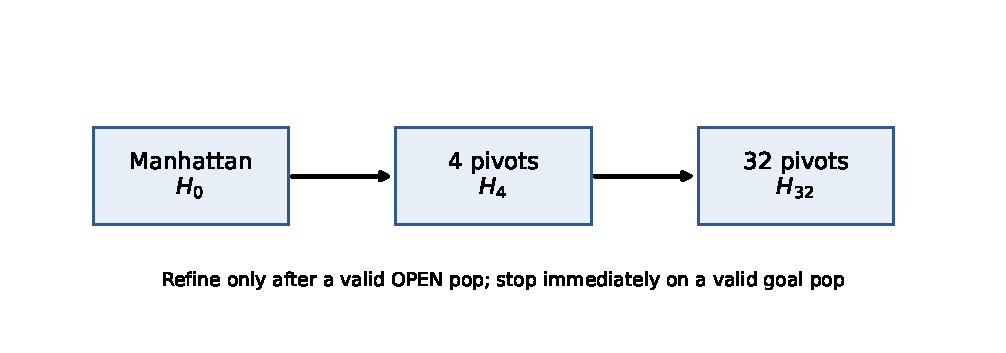
\includegraphics[width=\columnwidth]{stage_schematic.pdf}
  \caption{The proposed three-level staged-evaluation ladder.  A non-goal
  \Staged{} state expands only after reaching \HFull{}.}
  \label{fig:stages}
\end{figure}

\paragraph{\Manhattan.}
The start and every accepted state receive only \HMan{} and expand on a valid
pop.  This is the cheap, weak baseline.

\paragraph{\EagerFull.}
Every accepted state receives \HFull{} immediately.  This avoids heuristic
promotion and requeue overhead but pays all 32 landmark terms even for states
that never expand.

\paragraph{\LazyFull.}
Following Lazy \Astar{}, the start is fully evaluated before insertion.
Other accepted states initially receive \HMan{}.  A valid non-goal pop at the
cheap stage computes \HFull{} and requeues the state with the same insertion
ordinal; a later full-stage pop expands it.  A promotion occurs even when the
numeric estimate does not increase.

\paragraph{\Staged.}
The start computes \HPrefix{} and then the remaining 28 terms before its
initial insertion.  Other states begin with \HMan{}.  Their first valid
non-goal pop computes \HPrefix{} and requeues; a second competitive pop
computes only the remaining terms and requeues; a full-stage pop expands.
This method cannot bypass the suffix if a state is to expand.

\subsection{Shared graph-search contract}

OPEN entries are ordered lexicographically by
\begin{equation}
 (f,-g,\textit{ordinal},\textit{row-major id},
  \textit{version},\textit{stage}).
 \label{eq:open}
\end{equation}
A successful relaxation receives a fresh ordinal; heuristic promotion
preserves it.  Per-state labels store the best $g$, parent, version, ordinal,
completed stage, and current $h$.  Stale entries are discarded.  Cached
heuristic stages survive a later strict better-$g$ relaxation because their
values do not depend on $g$.  CLOSED reopening is implemented even though
consistency made its count zero in this experiment.

On a valid pop, the goal test precedes expensive refinement.  Every heuristic
is zero at the goal, so refinement could not raise its key.  A non-goal state
enumerates successors only at its condition's final stage.  We define
\emph{expanded} accordingly; the returned goal is not counted as expanded and
does not enter the expansion digest.

\subsection{Optimality and trace equivalence}

At every stage, $f=g+h$ is a lower bound on the cost of a solution through the
entry.  Suppose a goal with cost $C$ is validly popped.  If a cheaper solution
of cost $C'<C$ existed, some frontier state on that path would have a current
key at most $C'$.  If unrefined, it would be popped, refined to another lower
bound no greater than $C'$, and requeued; if fully refined, it would precede
the goal.  Either case contradicts the goal being minimal in OPEN.  Finite
maps, positive costs, stale-entry rejection, and reopening give completeness
for every valid query.

Moreover, \EagerFull{}, \LazyFull{}, and \Staged{} all expand non-goal states
only with the same \HFull{} value.  Promotion preserves ordinal, and
Equation~\ref{eq:open} fixes final-stage ordering.  Therefore they should
enumerate successors in the same sequence.  The implementation hashes that
sequence.  Digest equality is used as a fail-closed empirical invariant in
addition to the proof and independent BFS cost check.

Counters distinguish deterministic work from timing: expanded and generated
states, relaxations, pops, stale pops, requeues, calls to Manhattan/prefix/
suffix/full stages, pivot evaluations, table reads, cache hits, discovered
states, and maximum OPEN/live-state sizes.  Timing covers the complete search,
while per-stage timers are disabled to avoid instrumentation changing the
quantity measured.

\section{Experimental Protocol}
\label{sec:protocol}

\subsection{Map split and query selection}

The checksum-pinned source snapshot contains Moving AI pathfinding maps and
random scenario files \citep{sturtevant2012benchmarks}.  Table~\ref{tab:design}
summarizes the map-disjoint design.  The same four topology families occur on
both sides, but no map file overlaps.  Development uses one map per family and
40 queries per map to validate correctness, completeness, provenance, and the
analysis code; it performs no selection.  Evaluation begins only after an
external audit of those checks and uses two new maps per family with 100
queries per map.

\begin{table}[t]
\centering
\small
\caption{Experimental design.  Each query-method pair has one warm-up and eight
timed searches.}
\label{tab:design}
\begin{tabular}{lrrr}
\toprule
Split & Maps & Queries & Search runs \\
\midrule
Development & 4 & 160 & 5,760 \\
Sealed evaluation & 8 & 800 & 28,800 \\
\midrule
Total & 12 & 960 & 34,560 \\
\bottomrule
\end{tabular}
\end{table}

For each map, scenario files 1--4 are read in original source order.  A row is
valid when endpoints are distinct traversable cells in the same four-neighbor
component.  The plan takes the first 10 valid rows per file for development
and the first 25 for evaluation.  Duplicate $(\text{map},s,t)$ keys invalidate
the plan.  No query is sampled, replaced, or removed after timing.

The four development maps are
\texttt{maze-128-128-1}, \texttt{random-64-64-10},
\texttt{room-64-64-8}, and \texttt{warehouse-20-40-10-2-1}.
The evaluation's validation-source maps are
\texttt{maze-128-128-2}, \texttt{random-32-32-20},
\texttt{room-64-64-16}, and \texttt{warehouse-10-20-10-2-1};
its holdout-source maps are \texttt{maze-128-128-10},
\texttt{random-32-32-10}, \texttt{room-32-32-4}, and
\texttt{warehouse-10-20-10-2-2}.

\subsection{Balanced timing}

Within every query, the base method order is Manhattan, eager full, lazy full,
and staged.  One untimed warm-up uses that order.  Eight timed repetitions
left-rotate it by repetition index, cycling through the four positions twice.
Thus every method appears exactly twice in every position for every query.
Runs are sequential on one machine (Windows 11, CPython 3.12.9, 8 logical
CPUs); no concurrent search workers are used.

For a query and method, search time is the ordinary even median of eight
observations: the mean of the fourth and fifth sorted values.  Repetitions
reduce measurement noise and are not statistical units.  The primary
staged/lazy estimand is
\begin{equation}
 \exp\!\left(\operatorname{median}_{q}
     \log\frac{T_{q,\mathrm{staged}}}{T_{q,\mathrm{lazy}}}\right).
 \label{eq:ratio}
\end{equation}
Its percentile interval uses 10,000 deterministic bootstrap replicates
(seed 23725513), sampling maps first and then queries within sampled maps.
The eight maps are the top-level clusters.  Quartiles use Hyndman--Fan type 7.

\subsection{Validation and analysis}

All 800 records must be present, all costs must match replayed BFS, every path
must be legal, method summaries must match all repetitions, and the three
full-landmark expansion digests must agree.  Timing is analyzed only after all
checks pass.  There are no post-hoc exclusions.  Mechanism measures are exact per-query
counter differences.  Spearman associations use average ranks and are
descriptive.  Preprocessing amortization computes, within each map,
\begin{equation}
 A_m(Q)=\overline{T}_{m}+B_m/Q,
 \label{eq:amortization}
\end{equation}
where $B_m$ is measured landmark construction time and $Q$ is queries served;
the reported value equal-weights the eight maps.  Manhattan has $B_m=0$;
all landmark modes receive the same build charge.

\section{Results}
\label{sec:results}

\subsection{Integrity and hypothesis outcomes}

All 800 evaluation queries were retained.  Independent BFS and deterministic
search replay passed for every query; all four methods returned the BFS cost,
and \EagerFull{}, \LazyFull{}, and \Staged{} had matching full-landmark
expansion digests in all 800 cases.  No post-hoc exclusion was made.  These
checks passed before timing was analyzed.

\begin{table*}[t]
\centering
\small
\caption{Outcomes under the prespecified analysis.  H3 is descriptive;
its bootstrap fraction and correlation are not significance or causal tests.}
\label{tab:hypotheses}
\resizebox{\textwidth}{!}{\begin{tabular}{llll}
\toprule
Hypothesis & Status & Estimate & Interval \\
\midrule
H1 & passed & 800/800 queries passed both gates & not applicable (exact validation) \\
H2 & supported & pivot=0.0309758772; read=0.0301724138 & descriptive IQRs in summary/map tables \\
H3 & descriptive & ratio=1.05430023; Spearman rho=-0.640610853 & hierarchical bootstrap 95\% CI [0.989043253, 1.10158524] \\
\bottomrule
\end{tabular}
}
\end{table*}

Table~\ref{tab:hypotheses} reports the prespecified outcomes.  H2 was supported:
relative to \LazyFull{}, \Staged{} saved a median 3.0976\% of pivot
evaluations and 3.0172\% of table reads.  The corresponding query-level
medians were 28 fewer pivots/reads and one avoided suffix call, while the
median additional OPEN work was 116 combined queue operations (insertions and
pops).  Pivot-evaluation savings were nonnegative (420 positive, 380 zero) and
skewed: the median was 3.10\%, the mean 13.44\%, and the IQR 0--27.34\%.  This is a
heuristic-work improvement, not a wall-clock improvement.

\subsection{Search time and deterministic work}

The primary staged/lazy time ratio was 1.054300.  Its map-then-query
hierarchical bootstrap interval was $[0.989043,1.101585]$; 5.3\% of bootstrap
replicates had a ratio below one.  Since the interval includes one and only
eight top-level clusters are available, we make no categorical dominance or
significance claim.

\begin{table}[t]
\centering
\scriptsize
\caption{Overall per-query summaries on 800 evaluation queries.  Time is the
mean of each query's eight-run median, in ms; counters are query means.}
\label{tab:methods}
\begin{tabular}{lrrrrr}
\toprule
Method & Time & Expanded & Pops & Requeues & Reads \\
\midrule
Manhattan & 15.535 & 1197.86 & 1356.08 & 0.00 & 0.00 \\
Eager full & 8.149 & 160.69 & 162.09 & 0.00 & 9977.68 \\
Lazy full & 8.282 & 160.69 & 422.15 & 260.06 & 8385.88 \\
Staged & 8.056 & 160.69 & 599.86 & 437.78 & 6080.29 \\
\bottomrule
\end{tabular}
\end{table}

Table~\ref{tab:methods} exposes the tradeoff.  All full-landmark schedules
averaged 160.69 expansions and 517.30 generated successors per query,
compared with 1197.86 and 4043.00 for Manhattan.  Eager evaluation minimized
OPEN operations but averaged 9,945.68 pivot evaluations.  Ordinary lazy
evaluation reduced this to 8,353.88 at the cost of 260.06 requeues.  Staging
reduced it further to 6,048.29 but averaged 437.78 requeues and 599.86 pops.
No method reopened a state.  Table~\ref{tab:methods} averages query medians,
whereas the primary statistic is a median of paired time ratios.  These are
different estimands, especially under strong map heterogeneity.

\subsection{Map and family crossover}

\begin{figure}[t]
  \centering
  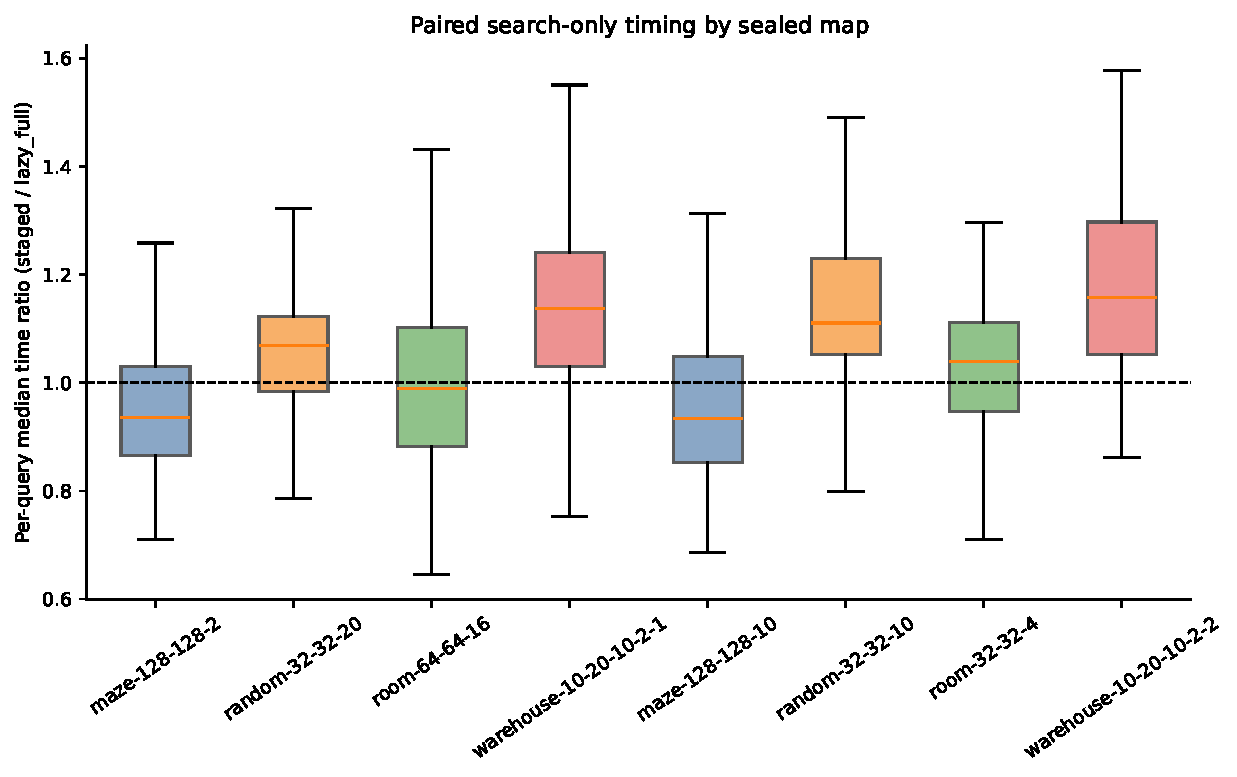
\includegraphics[width=\columnwidth]{per_map_time_ratios.pdf}
  \caption{Per-map distributions of paired staged/lazy search-time ratios.
  The horizontal reference at one denotes equal time.}
  \label{fig:map-ratios}
\end{figure}

\begin{table}[t]
\centering
\scriptsize
\caption{Per-map medians.  Ratio $<1$ favors staged evaluation; read saving is
relative to ordinary lazy evaluation.  V and H denote validation- and
holdout-source maps.}
\label{tab:maps}
\begin{tabular}{llrr}
\toprule
Family & Source/map & Time ratio & Read saving \\
\midrule
Maze & V: 128-2 & 0.935 & 31.17\% \\
Maze & H: 128-10 & 0.934 & 30.34\% \\
Random & V: 32-20 & 1.069 & 2.50\% \\
Random & H: 32-10 & 1.110 & 0.00\% \\
Room & V: 64-16 & 0.990 & 18.47\% \\
Room & H: 32-4 & 1.039 & 11.46\% \\
Warehouse & V: 10-20-1 & 1.137 & 0.00\% \\
Warehouse & H: 10-20-2 & 1.157 & 0.00\% \\
\bottomrule
\end{tabular}
\end{table}

Figure~\ref{fig:map-ratios} and Table~\ref{tab:maps} show repeatable family
regimes.  Both maze maps saved about 30--31\% of reads and favored staging by
about 6.5\%.  Both warehouse maps had zero median read saving and favored
ordinary lazy evaluation by 13.7--15.7\%.  Random maps favored lazy, while the
two room maps lay on opposite sides of one.  The same direction on the two
maze and two warehouse maps is suggestive replication within those families,
not a population-level guarantee.

\begin{figure*}[t]
  \centering
  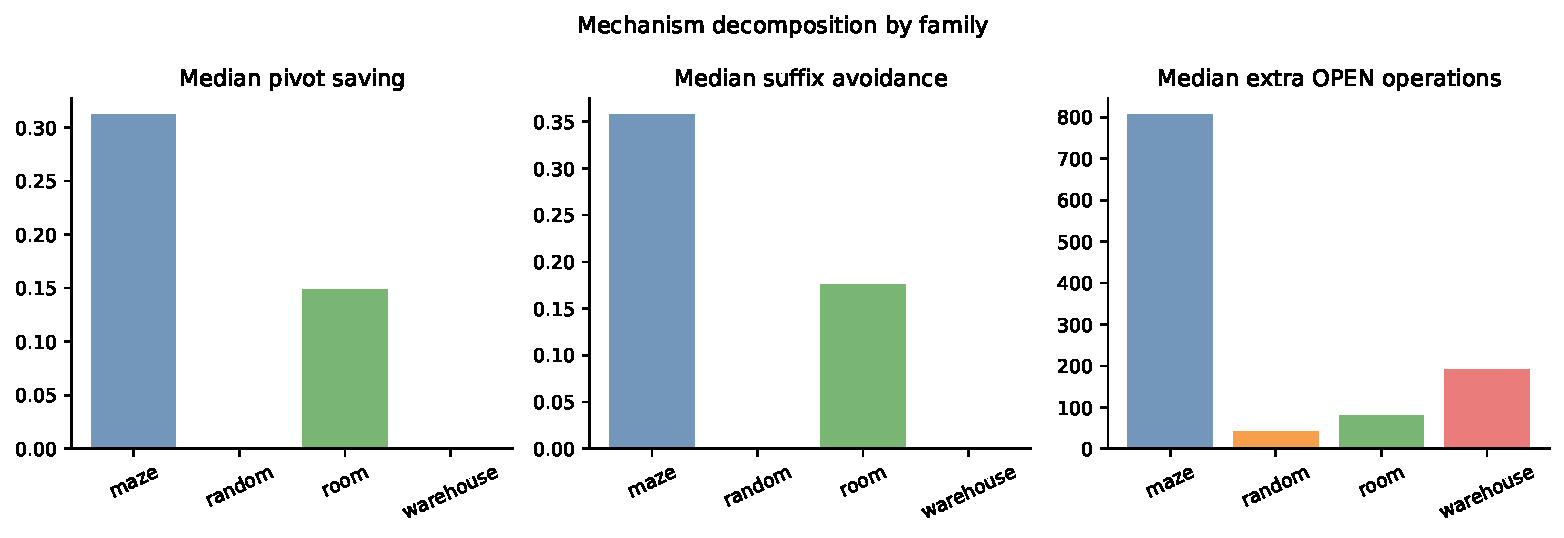
\includegraphics[width=0.92\textwidth]{family_mechanism_decomposition.pdf}
  \caption{Family-level decomposition of saved landmark work and added OPEN
  work.  Families are equal-weighted through their constituent queries.}
  \label{fig:families}
\end{figure*}

\begin{figure*}[t]
  \centering
  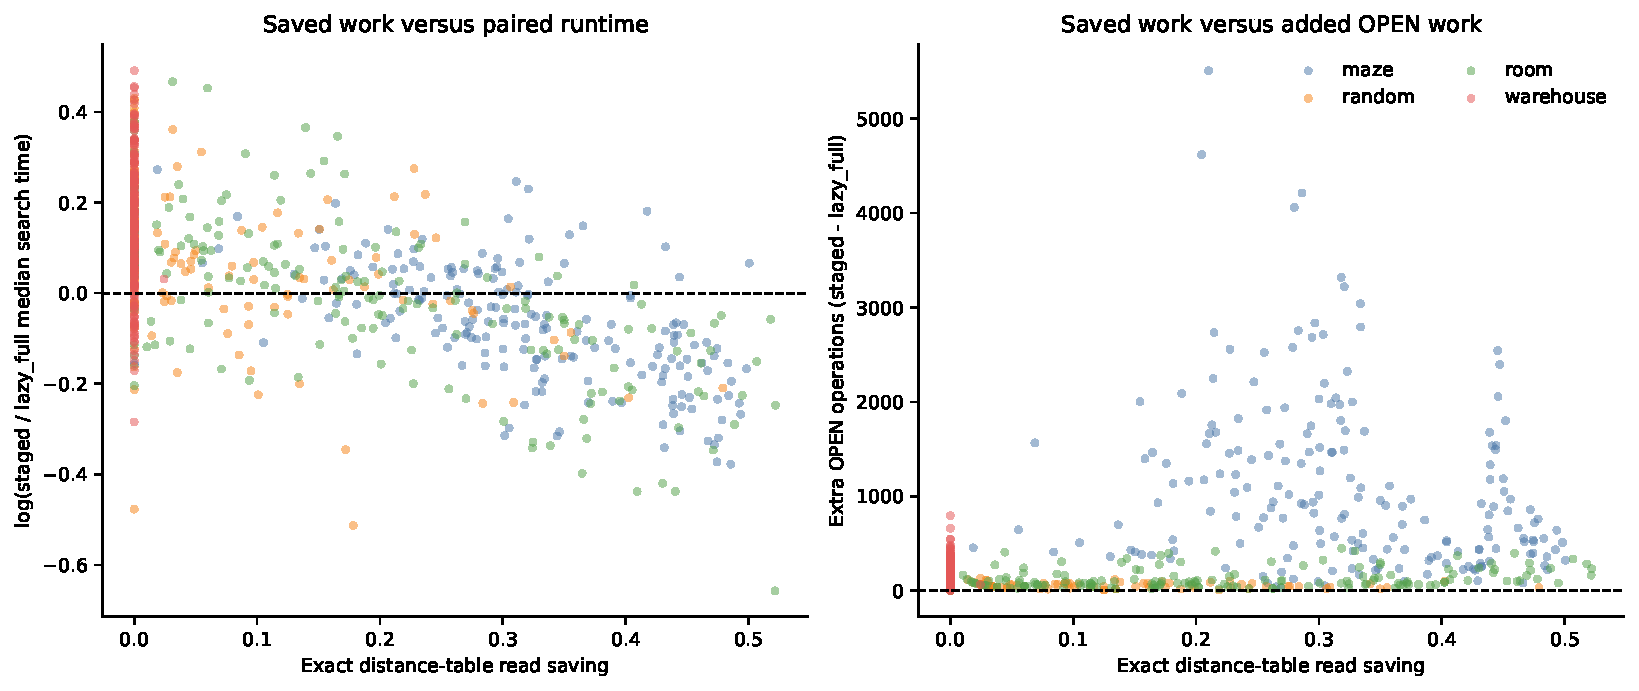
\includegraphics[width=0.92\textwidth]{saved_work_vs_time.pdf}
  \caption{Query-level exact work changes versus paired time ratio.  The
  association is descriptive and queries within a map are dependent.}
  \label{fig:saved-work}
\end{figure*}

Across all 800 queries, read-saving fraction and log time ratio had Spearman
$\rho=-0.640611$; extra OPEN work and log ratio had $\rho=-0.240994$.
Figure~\ref{fig:saved-work} makes the crossover visible but does not isolate a
causal coefficient: difficulty, topology, and absolute search size affect both
the counters and time.

\subsection{Preprocessing amortization}

\begin{figure}[t]
  \centering
  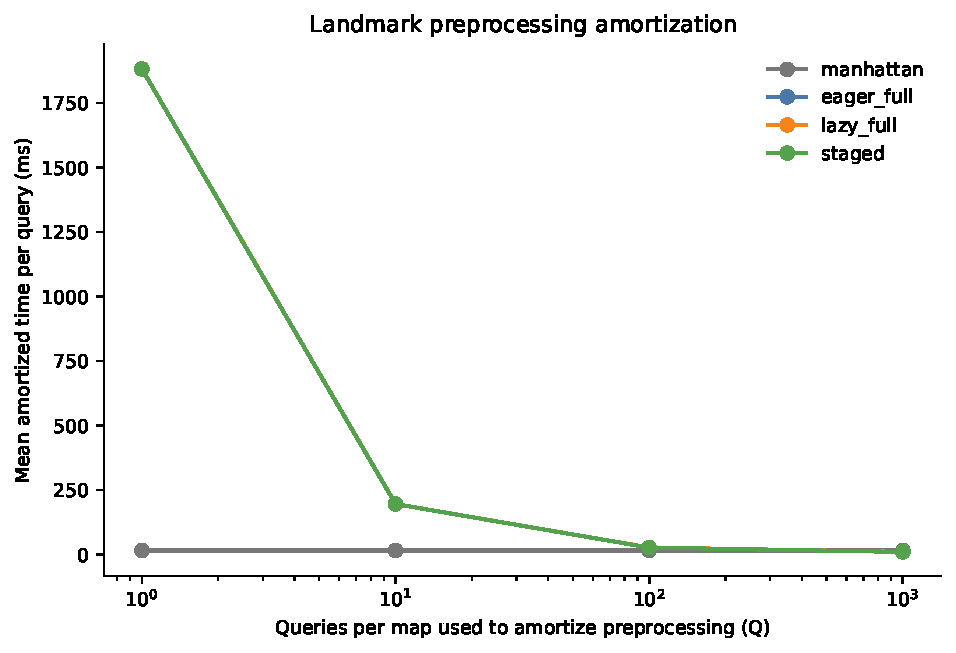
\includegraphics[width=\columnwidth]{preprocessing_amortization.pdf}
  \caption{Equal-map-weighted amortized time as the one-time 32-landmark table
  construction is spread over $Q$ queries.}
  \label{fig:amortization}
\end{figure}

\begin{table}[t]
\centering
\scriptsize
\caption{Mean amortized ms/query, equal-weighting eight maps.}
\label{tab:amortization}
\begin{tabular}{rrrrr}
\toprule
$Q$ & Manhattan & Eager & Lazy & Staged \\
\midrule
1 & 15.535 & 1881.862 & 1881.995 & 1881.769 \\
10 & 15.535 & 195.520 & 195.653 & 195.427 \\
100 & 15.535 & 26.886 & 27.019 & 26.793 \\
1000 & 15.535 & 10.023 & 10.155 & 9.929 \\
\bottomrule
\end{tabular}
\end{table}

Preprocessing dominates when a table serves few queries
(Figure~\ref{fig:amortization}, Table~\ref{tab:amortization}).  At $Q=100$ all
landmark modes remain slower than Manhattan after charging construction;
at $Q=1000$ they are faster under this equal-map average.  Because all three
landmark schedules share exactly the same table, preprocessing barely changes
their relative order; it changes the practical comparison with Manhattan.

\section{Discussion}
\label{sec:discussion}

\paragraph{RQ1: controlled correctness.}
The correctness and invariance gate passed without exceptions.  Cost equality
alone would allow subtle scheduling differences to remain hidden.  Identical
full-landmark expansion digests additionally show that eager, lazy, and staged
conditions performed the same successor-enumerating search under the frozen
tie breaker.  Their differences in time and counters can therefore be
localized to evaluation timing and OPEN promotions rather than to different
expanded state sets.

\paragraph{RQ2: staging saved real work.}
The prefix was not merely ceremonial.  Staging reduced median pivot and read
work by about 3\%, and much more on maze queries.  In operational terms,
\LazyFull{} evaluates all 32 terms whenever a cheap state becomes competitive;
\Staged{} spends four reads first and avoids the other 28 when that prefix
pushes the state below competitors.  The saving is exact and deterministic.
It is also heterogeneous and often zero, so the overall median understates
large savings in one regime and overstates the effect in another.

\paragraph{RQ3: saved work did not imply universal speed.}
Every intermediate evaluation requires another pop and requeue.  The staged
schedule averaged roughly 178 more requeues and 178 more pops per query than
ordinary lazy evaluation.  Its primary paired ratio of 1.0543 therefore points toward
a modest slowdown at the pooled median, while the 95\% interval includes
parity.  We interpret this as bounded negative evidence for universal use of
this fixed prefix, not as proof that staging can never help.  Indeed, the maze
maps show the expected positive regime.

The strong negative Spearman association between read saving and log time
ratio supports the proposed mechanism descriptively: queries that avoided a
larger fraction of reads tended to make staging relatively faster.  It cannot
establish that removing a particular read would cause the measured speedup.
Both variables co-vary with topology, query length, absolute number of
competitive nodes, cache locality, and Python priority-queue costs.

\paragraph{RQ4: topology and workload matter.}
Warehouses are the clearest failure regime.  The four-pivot prefix had zero
median saving on both maps, so it added a nearly pure heap cycle before the
same suffix work.  Mazes are the clearest success regime: the prefix filtered
enough candidates to save about 30\% of reads on both maps, outweighing
promotion overhead.  Random and room maps occupy intermediate or mixed
regimes.  This crossover is more informative than a single leaderboard rank:
it specifies when the simple schedule's mechanism is active.

Landmark construction changes the deployment decision at a different level.
If a map receives only a few queries, even a fast landmark search cannot repay
dozens of BFS preprocessing passes.  At high query volume the fixed cost is
small per query, and all landmark modes beat Manhattan under the study's
equal-map average.  The analysis deliberately charges the same build cost to
eager, lazy, and staged modes because they use the same table; staging is a
query-time schedule, not a preprocessing improvement.

\paragraph{Relation to prior work.}
The results instantiate the tradeoff identified by Lazy \Astar{}: heuristic
calls saved on surplus nodes versus extra OPEN manipulation
\citep{tolpin2013towards}.  They do not imply an optimal deployment policy and
do not challenge rational or learned methods, which may choose conditionally
whether to evaluate \citep{karpas2018rational,domshlak2012online}.  A natural
extension would use predecision features to choose between ordinary lazy and
staged schedules.  That is intentionally future work: fitting such a selector
after seeing these maps would change the question and require a new split.

\section{Limitations and Threats to Validity}
\label{sec:limitations}

\paragraph{Statistical scope.}
The evaluation has 800 queries but only eight top-level map clusters.  The
hierarchical bootstrap respects this structure, yet eight maps cannot support
precise population claims.  Two maps per family show useful within-family
replication, not coverage of all instances in that family.  The 0.053
bootstrap fraction is descriptive, not a $p$-value, and the interval is not
evidence of equivalence.

\paragraph{External validity.}
All problems are undirected, unit-cost, four-neighbor grids from four known
families.  Results may change on weighted or directed graphs, road networks,
diagonal movement, dynamic tasks, or other pivot-distance representations.
Families occur on both sides of the map-disjoint split, so this tests new maps
within known families rather than unseen-domain generalization.

\paragraph{Fixed design choices.}
$K=4$, $M=32$, and deterministic farthest-first placement form one prespecified
configuration.  The prefix may be unusually informative in some topologies
and redundant in others.  We did not compare alternate prefix sizes, pivot
orders, compression, adaptive stopping, or active-landmark techniques.  This
restriction prevents tuning to the evaluation maps but limits the conclusions to
the specified schedule.

\paragraph{Implementation and measurement.}
Packed-array reads and priority-queue operations have Python- and
hardware-specific costs.  Short searches remain sensitive to OS scheduling,
cache state, allocator behavior, and timer resolution despite a warm-up,
balanced order positions, and eight-run medians.  Disabling stage timers
avoids one perturbation but prevents assigning nanoseconds cleanly to prefix,
suffix, and heap operations.  Exact counters are more portable than runtime
crossover points.

\paragraph{Internal validity.}
A shared engine and trace digest greatly reduce implementation confounds, but
they also share any common bug.  Independent BFS, legal-path validation,
exhaustive small-map tests, immutable source hashes, deterministic replays,
and strict artifact loaders provide independent layers.  Expansion-trace
equality is an implementation invariant under the specified tie breaker; it is
not a general theorem that every Lazy \Astar{} implementation must duplicate
eager order.

\paragraph{Novelty.}
Every algorithmic ingredient has close prior art.  ALT and differential
heuristics establish landmark bounds; subset work establishes that a fixed
selection can trade evaluation cost and informativeness; Lazy \Astar{}
establishes delayed evaluation and notes straightforward multi-stage
extension.  This experiment studies their intersection.  A targeted search
found no exact match, although differently named or unpublished work may
exist.

\paragraph{Analysis rerun.}
The first complete development/evaluation attempt is preserved separately.
Before statistical output was produced, analysis stopped on a representation
mismatch: the loaded schedule used tuples while the equivalent JSON plan used
lists.  We normalized the container types, added a regression test, and reran
the full experiment because the analysis source hash had been fixed before the
first run.  The algorithm, protocol, queries, $K/M$ values, and estimands were
unchanged.  The 800 deterministic summaries match the first attempt; only
timings were remeasured.  The correction was not prompted by the observed
performance.

\section{Reproducibility and Provenance}
\label{sec:reproducibility}

Exact experiment and figure-generation code, configuration, source manifests,
frozen raw results, and analysis are preserved at:

\begin{center}
\fbox{\parbox{0.92\columnwidth}{\centering
\textbf{BLOCKER: INSERT PUBLIC REPOSITORY URL AND COMMIT SHA}}}
\end{center}

The authoritative configuration is
\path{configs/progressive_landmarks_v2.json} (SHA-256 prefix
\texttt{850176ee1990}); its canonical plan hash begins
\texttt{01aa82ec3984}.  The reported raw bundle is exclusively
\path{data/results/progressive_landmarks_v2_rerun1}; the sealed manifest binds
800 query records and 28,800 search runs.  The analysis directory is
\path{data/processed/progressive_landmarks_analysis_v2}; its manifest binds 800
query rows, eight map rows, summary/provenance files, and ten plots.  The
generated analysis summary hash begins \texttt{0f6e9fc457c3}.

The root \path{README.md} gives the exact copy-pasteable commands and arguments.
Their fixed order is: (1) verify the protocol with
\path{scripts/verify_progressive_landmarks_protocol.py}; (2) run development
with \path{scripts/run_progressive_landmarks.py}; (3) audit and freeze it with
\path{scripts/freeze_progressive_landmarks_development.py}; (4) invoke the same
runner for sealed evaluation while supplying that freeze; and (5) generate all
statistics and figures with \path{scripts/analyze_progressive_landmarks.py}.
Every command binds the v2 configuration and repository root.  The final three
stages also bind the development directory, audit, freeze, sealed directory,
and analysis directory named above, so a superseded or substituted artifact
fails closed.

Output directories are write-once and published atomically.  Manifests bind
file sizes, record counts, schemas, and SHA-256 hashes.  Formal loading replays
the canonical query plan, source maps, landmark tables, BFS oracle, paths,
method summaries, counters, and expansion digests instead of trusting
coherently edited stored fields.  The development audit records
\texttt{selection\_performed=false}; its freeze is required to authorize
sealed evaluation.  Analysis again validates that authorization and all
correctness gates before reading timing.

The report figures are byte-for-byte copies of the analysis PDFs.  The
hypothesis table is the generated \LaTeX{} fragment rather than a manually
retyped result.  Compact method, map, and amortization tables were transcribed
only from the immutable summary JSON and map CSV and are cross-checked in the
report audit.  Build the paper from \texttt{report/} with
\texttt{pdflatex}, \texttt{bibtex}, and two final \texttt{pdflatex} passes.

\section{Conclusion}
\label{sec:conclusion}

Progressively evaluating a fixed differential-landmark prefix is correct and
can avoid substantial heuristic work, but the additional OPEN cycle is not
free.  Under the locked $4\rightarrow32$ schedule, staging saved a median
3.10\% of pivot evaluations and 3.02\% of distance reads, while its primary
paired time ratio relative to ordinary Lazy \Astar{} was 1.0543 with a 95\%
hierarchical bootstrap interval of $[0.9890,1.1016]$.  The pooled result does
not support a universal speed advantage.

The map regimes answer the more useful question.  A four-pivot prefix helped
on mazes, where it removed about 30\% of reads and both maps favored staging.
It hurt on warehouses, where median read saving was zero and both maps favored
ordinary lazy evaluation.  Thus the relevant condition is whether the prefix
filters enough full evaluations to repay its extra pops and requeues.  That
finding is descriptive and implementation-conditional, but it is supported by
exact work counters, a negative read-saving/time-ratio association, independent
BFS validation, and identical full-landmark expansion traces.

The study's scientific value lies in disciplined scope: it combines familiar
course concepts into a reproducible experiment, states an honest prior-art
boundary, preserves a sealed map-disjoint protocol, and reports a mixed result
rather than tuning it away.  Future work could preregister multiple prefix
sizes or a deployment selector on new maps, port the engine to a lower-level
language, and test weighted or directed graphs.  Those extensions require new
data and are not inferred from this evaluation.


\enlargethispage{2\baselineskip}
\bibliography{../references/references}

\end{document}
